\documentclass{article}
\usepackage[utf8]{inputenc}
\usepackage[english]{babel}
\usepackage{algorithm}
\usepackage{algorithmicx}
\usepackage{listings}
\usepackage{graphicx}
\usepackage{vmargin}
\usepackage[noend]{algpseudocode}
\usepackage{listings}
\usepackage{color}
\usepackage[dvipsnames]{xcolor}
\usepackage{esvect}
\usepackage[spanish]{babel}
\usepackage[latin1]{inputenc}
\usepackage[usenames]{color}
\definecolor{backgroundColour}{rgb}{0.95,0.95,0.92}
\definecolor{mGreen}{rgb}{0,0.6,0}
\definecolor{mPurple}{rgb}{0.58,0,0.82}
\usepackage{hyperref}
\usepackage{amsmath}
\usepackage{esint}

\lstset{ 
	language=Matlab,                		
%	basicstyle=10pt,       			
	numbers=left,                  		
	numberstyle=\footnotesize,      		
	stepnumber=1,                   		
	numbersep=5pt,                  	
	backgroundcolor=\color{backgroundColour},
	commentstyle=\color{mGreen},
	keywordstyle=\color{blue},
	stringstyle=\color{mPurple},
	showspaces=false,               		
	showstringspaces=false,         		
	showtabs=false,                 			
%	tabsize=2,                			
%	captionpos=b,                   		
	breaklines=true,                			
	breakatwhitespace=false,        		
	escapeinside={\%*}{*)}          	
}


\usepackage{enumitem}

\setmargins{2.0cm}      % margen izquierdo
{1cm}                   % margen superior
{17cm}                  % anchura del texto
{23.42cm}               % altura del texto
{0cm}                   % altura de los encabezados
{1cm}                   % espacio entre el texto y los encabezados
{0cm}                   % altura del pie de página
{1cm}                   % espacio entre el texto y el pie de página


\title{
    Universidad Nacional de San Agustín 
    \\
    \large Escuela de Ingeniería de Sistemas
    \\
    \rule{100mm}{0.1mm}
    \\
    \huge Práctica 9
    \\
    \large Física Computacional

    \\
    \rule{100mm}{0.5mm}
    }
\author{Carlos Alberto Mestas Escarcena}
\date{Julio 2020}

\begin{document}

\maketitle
El desarrollo de este informe se puede encontrar en el repositorio de \textcolor{blue}{
    \href{https://github.com/CarlosMestas/FC_CarlosMestas_Practica9}{GitHub}}.

\section{Evalúe el área de la elipse en el primer cuadrante}

\begin{lstlisting} [frame=single]
clear, clf, hold off
m = 100000; veces = 50;
ax = 0; bx  = 2;
ay = 0; by  = 3;
sa = 0; saa = 0;
for k=1:veces
    n=0;
    for i=1:m
        r = rand; x = ax + (bx-ax)*r;
        r = rand; y = ay + (by-ay)*r;
        if (x^2/4+y^2/9) < 1
            n     = n+1;
            px(n) = x; 
            py(n) = y;
        end
    end
    area = n*(by-ay)*(bx-ax)/m;
    sa   = sa + area;
    saa  = saa + area^2;
end
prom = sa/veces;
desv = sqrt(veces*saa-sa^2)/veces;
promedio = num2str(prom);
desviacion = num2str(desv);
plot (px,py,'.'),
title('Áreas por el metodo MonteCarlo') 
xlabel('x');
ylabel('y');
axis equal;
axis([ax-0.1,bx+0.1,ay-0.1,by+0.1])
text(ax/2+0.5+bx/2,by-0.25,promedio);
text(ax/2+0.5+bx/2,by-0.50,'+-');
text(ax/2+0.5+bx/2,by-0.75,desviacion);
\end{lstlisting}

\begin{figure}[H]
\centering
    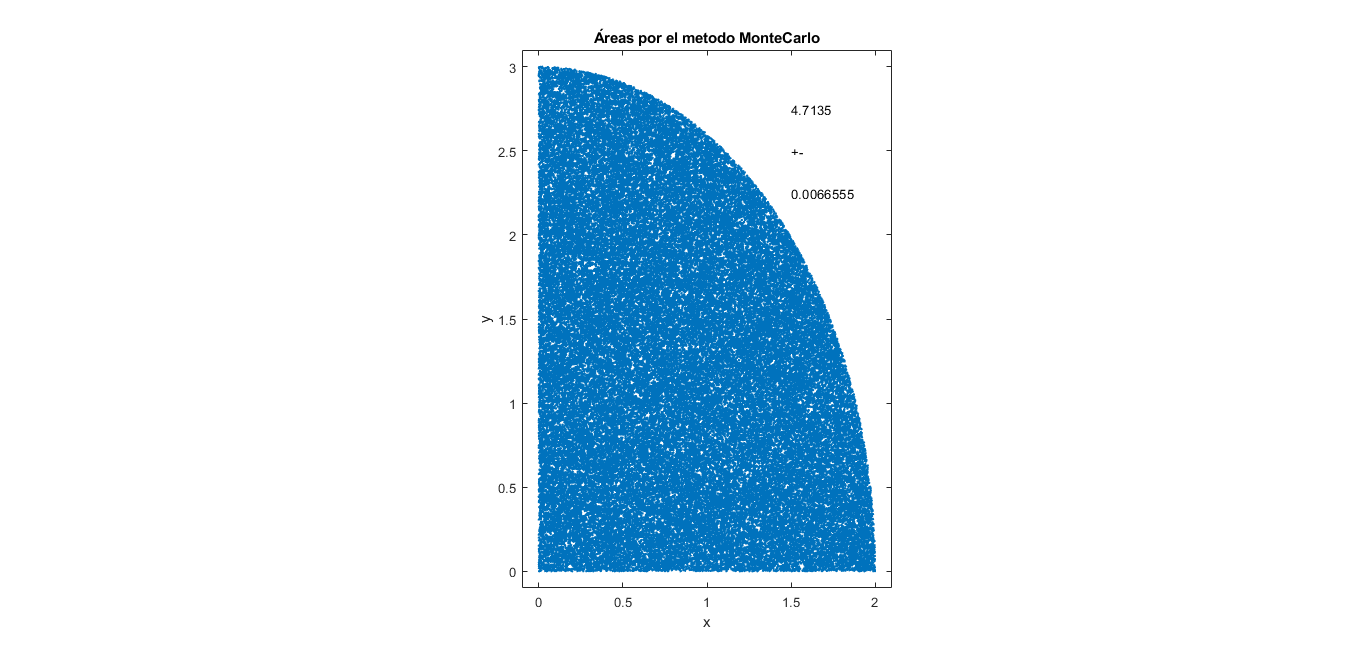
\includegraphics[width=1\textwidth]{images/FIG01.png}
    \caption{Área de la eclipse en el primer cuadrante}
\end{figure}
El área de la sección es = $4.7135~+/-~0.0066555$



\section{Evalúe las siguientes integrales}

\subsection{A}

\begin{equation}
I = \int_{0}^{1} exp(x^2)~dx
\end{equation}

\begin{lstlisting} [frame=single]
clear, clf, hold off
m = 100000; veces = 50;
ax = 0; bx  = 1;
ay = 0; by  = 3;
sa = 0; saa = 0;
for k=1:veces
    n=0;
    for i=1:m
        r = rand; x = ax + (bx-ax)*r;
        r = rand; y = ay + (by-ay)*r;
        if (y < exp(x^2)) && (y > 0) && (x > 0) && (x < 1)
            n     = n+1;
            px(n) = x; 
            py(n) = y;
        end
    end
    area = n*(by-ay)*(bx-ax)/m;
    sa   = sa + area;
    saa  = saa + area^2;
end
prom = sa/veces;
desv = sqrt(veces*saa-sa^2)/veces;
promedio = num2str(prom);
desviacion = num2str(desv);
plot (px,py,'.'),
title('Áreas por el metodo MonteCarlo') 
xlabel('x');
ylabel('y');
set(gcf, 'Position', get(0, 'Screensize'));
axis equal;
axis([ax-0.1,bx+0.1,ay-0.1,by+0.1])
text(ax/2+bx/2,by-0.25,promedio);
text(ax/2+bx/2,by-0.50,'+-');
text(ax/2+bx/2,by-0.75,desviacion);
\end{lstlisting}

\begin{figure}[H]
\centering
    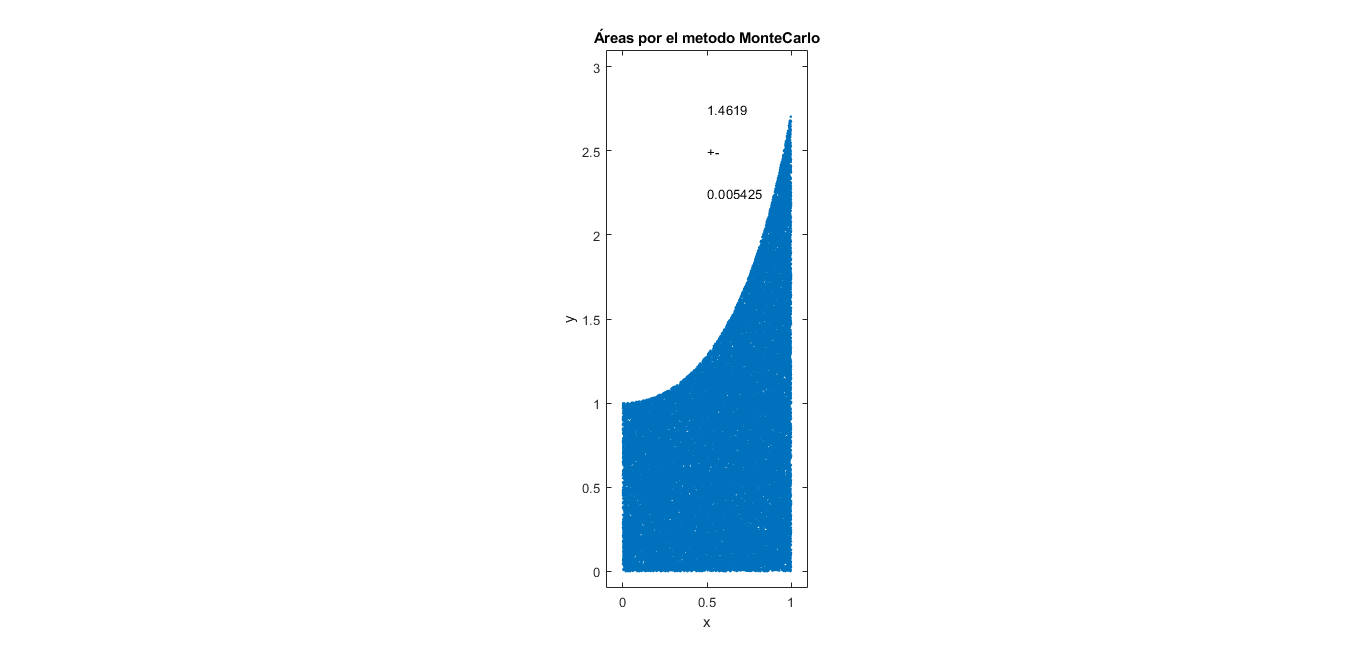
\includegraphics[width=1\textwidth]{images/FIG02A.png}
    \caption{Área de la sección}
\end{figure}
El área de la sección es = $4.7135~+/-~0.0066555$

\subsection{B}

\begin{equation}
I = \int_{1}^{3} \sqrt{x^3-1}~dx
\end{equation}

\begin{lstlisting} [frame=single]
clear, clf, hold off
m = 100000; veces = 50;
ax = 0; bx  = 1;
ay = 0; by  = 3;
sa = 0; saa = 0;
for k=1:veces
    n=0;
    for i=1:m
        r = rand; x = ax + (bx-ax)*r;
        r = rand; y = ay + (by-ay)*r;
        if (y <= exp(x^2)) && (x > 0) && (x < 1)
            n     = n+1;
            px(n) = x; 
            py(n) = y;
        end
    end
    area = n*(by-ay)*(bx-ax)/m;
    sa   = sa + area;
    saa  = saa + area^2;
end
prom = sa/veces;
desv = sqrt(veces*saa-sa^2)/veces;
promedio = num2str(prom);
desviacion = num2str(desv);
plot (px,py,'.'),
title('Áreas por el metodo MonteCarlo') 
xlabel('x');
ylabel('y');
axis equal;
axis([ax-0.1,bx+0.1,ay-0.1,by+0.1])
text(ax/2+bx/2,by-0.25,promedio);
text(ax/2+bx/2,by-0.50,'+-');
text(ax/2+bx/2,by-0.75,desviacion);
\end{lstlisting}

\begin{figure}[H]
\centering
    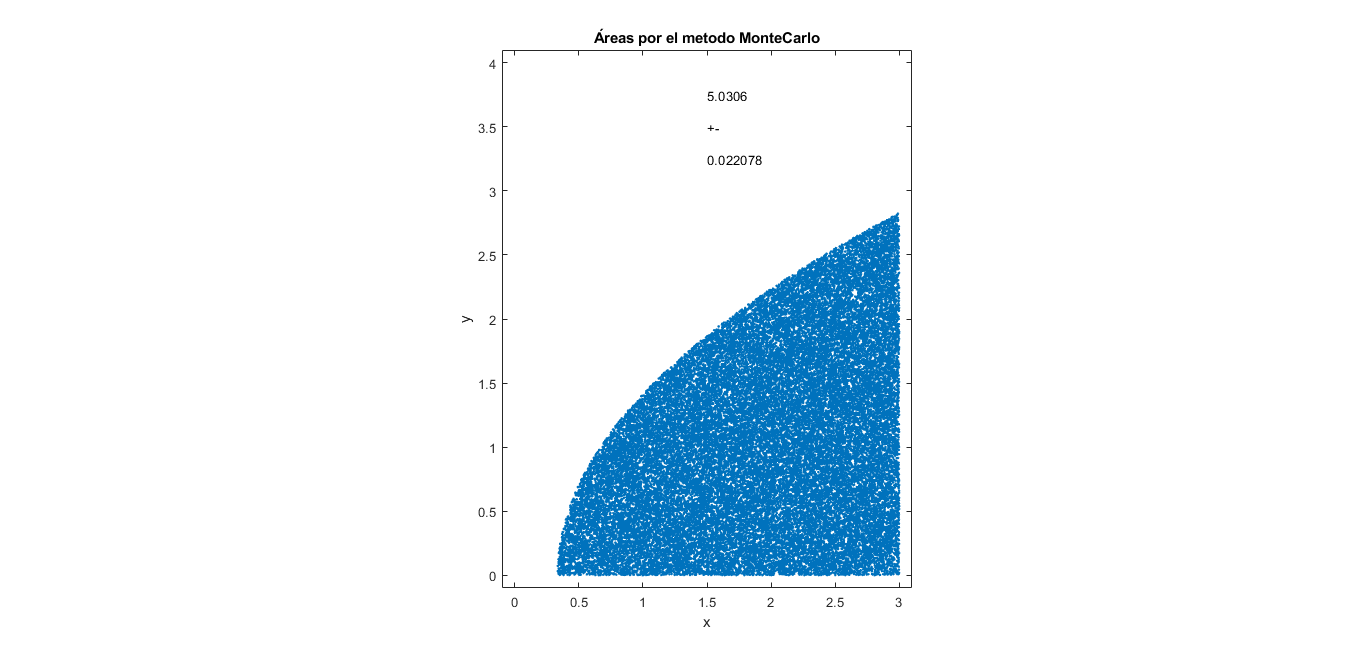
\includegraphics[width=1\textwidth]{images/FIG02B.png}
    \caption{Área de la sección}
\end{figure}

\section{Calcule el área de la figura limitada por las líneas cuyas ecuaciones son}

\begin{equation}
y^2=2x+1
\end{equation}
\begin{equation}
x-y-1=0
\end{equation}

Primero realizaremos las gráficas de las líneas para darnos una idea de lo que vamos a obtener en el código:

\clearpage
\newpage

\begin{figure}[H]
\centering
    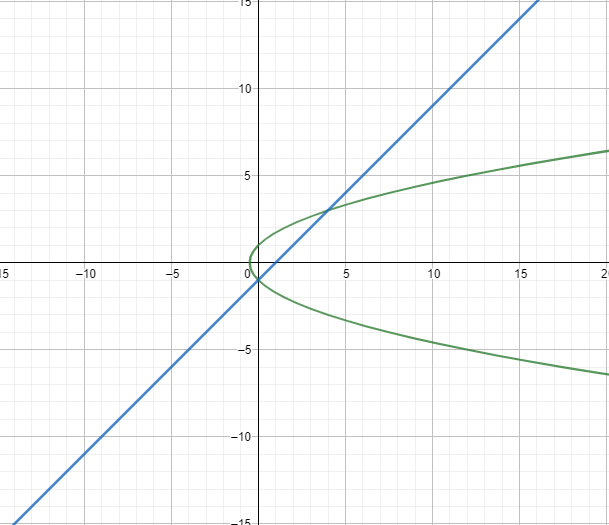
\includegraphics[width=0.5\textwidth]{images/Capture03.PNG}
    \caption{Gráfica de las líneas para delimitar el área del ejercicio 3}
\end{figure}

\begin{lstlisting} [frame=single]
clear, clf, hold off
m = 100000; veces = 50;
ax = -1; bx  = 5;
ay = -2; by  = 4;
sa = 0; saa = 0;
for k=1:veces
    n=0;
    for i=1:m
        r = rand; x = ax + (bx-ax)*r;
        r = rand; y = ay + (by-ay)*r;
        if (-y^2+2*x+1>=0) && (x - y - 1 <= 0)
            n     = n+1;
            px(n) = x; 
            py(n) = y;
        end
    end
    area = n*(by-ay)*(bx-ax)/m;
    sa   = sa + area;
    saa  = saa + area^2;
end
prom = sa/veces;
desv = sqrt(veces*saa-sa^2)/veces;
promedio = num2str(prom);
desviacion = num2str(desv);
plot (px,py,'.'),
title('Áreas por el metodo MonteCarlo') 
xlabel('x');
ylabel('y');
axis equal;
axis([ax-0.1,bx+0.1,ay-0.1,by+0.1])
text(ax/2+bx/2,by-0.25,promedio);
text(ax/2+bx/2,by-0.50,'+-');
text(ax/2+bx/2,by-0.75,desviacion);
\end{lstlisting}

\clearpage
\newpage

\begin{figure}[H]
\centering
    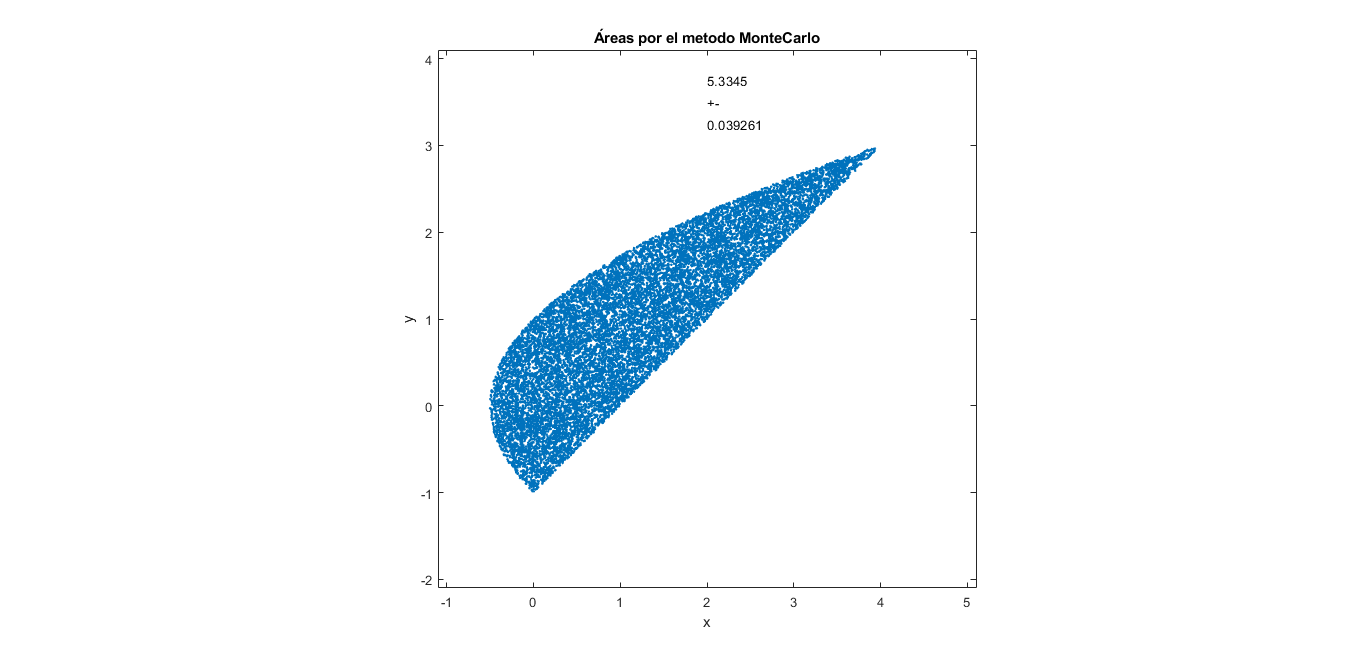
\includegraphics[width=1\textwidth]{images/FIG03.png}
    \caption{Área de la sección}
\end{figure}
El área de la sección es = $5.3345~+/-~0.039261$

\section{Calcule el área de la figura limitada por las parábolas}

\begin{equation}
y=x^2
\end{equation}
\begin{equation}
y=\sqrt{x}
\end{equation}

Primero realizaremos las gráficas de las líneas para darnos una idea de lo que vamos a obtener en el código:

\begin{figure}[H]
\centering
    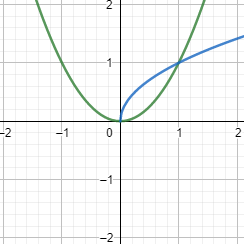
\includegraphics[width=0.5\textwidth]{images/Capture04.PNG}
    \caption{Gráfica de las líneas para delimitar el área del ejercicio 4}
\end{figure}

\clearpage
\newpage

\begin{lstlisting} [frame=single]
clear, clf, hold off
m = 100000; veces = 50;
ax = 0; bx  = 1;
ay = 0; by  = 1;
sa = 0; saa = 0;
for k=1:veces
    n=0;
    for i=1:m
        r = rand; x = ax + (bx-ax)*r;
        r = rand; y = ay + (by-ay)*r;
        if (y<=x^0.5) && (y>x^(2))
            n     = n+1;
            px(n) = x; 
            py(n) = y;
        end
    end
    area = n*(by-ay)*(bx-ax)/m;
    sa   = sa + area;
    saa  = saa + area^2;
end
prom = sa/veces;
desv = sqrt(veces*saa-sa^2)/veces;
promedio = num2str(prom);
desviacion = num2str(desv);
plot (px,py,'.'),
title('Áreas por el metodo MonteCarlo') 
xlabel('x');
ylabel('y');
axis equal;
axis([ax-0.1,bx+0.1,ay-0.1,by+0.1])
text(ax/2+bx/2+0.25,by-0.25-0.25,promedio);
text(ax/2+bx/2+0.25,by-0.50-0.25,'+-');
text(ax/2+bx/2+0.25,by-0.75-0.25,desviacion);
\end{lstlisting}

\begin{figure}[H]
\centering
    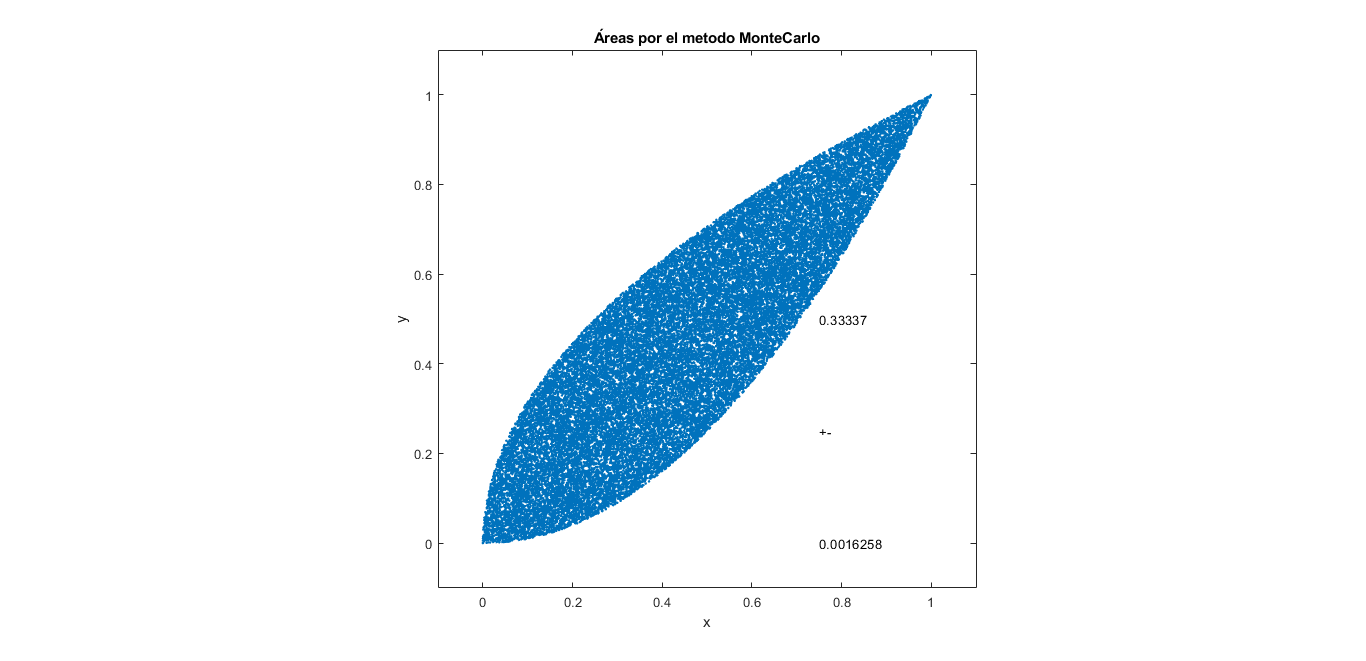
\includegraphics[width=1\textwidth]{images/FIG04.png}
    \caption{Área de la sección}
\end{figure}
El área de la sección es = $0.33337~+/-~0.0016258$

\section{Encuentre el volumen de un elipsoide}

\begin{lstlisting} [frame=single]
clear, clf, hold off
m = 100000; veces = 50;
ax = -4; bx  = 4;
ay = -3; by  = 3;
az = -2; bz  = 2; 
sa = 0; saa = 0;
for k=1:veces
    n=0;
    for i=1:m
        r = rand; x = ax + (bx-ax)*r;
        r = rand; y = ay + (by-ay)*r;
        r = rand; z = az + (bz-az)*r;
        if (x^2/16+y^2/9+z^2/4) < 1
            n     = n+1;
            px(n) = x; 
            py(n) = y;
            pz(n) = z;
        end
    end
    volumen = n*(by-ay)*(bx-ax)*(bz-az)/m;
    sa   = sa + volumen;
    saa  = saa + volumen^2;
end
prom = sa/veces;
desv = sqrt(veces*saa-sa^2)/veces;
promedio = num2str(prom);
desviacion = num2str(desv);
plot3(px,py,pz,'.'),
title('Áreas por el metodo MonteCarlo') 
xlabel('x');
ylabel('y');
zlabel('z');
axis equal;
axis ([ax-0.1,bx+0.1,ay-0.1,by+0.1,az-0.1,bz+0.1]);
text(ax/2+bx/2,by-0.25+bz-0.25,promedio);
text(ax/2+bx/2,by-0.50+bz-0.25,'+-');
text(ax/2+bx/2,by-0.75+bz-0.25,desviacion);
\end{lstlisting}

\begin{figure}[H]
\centering
    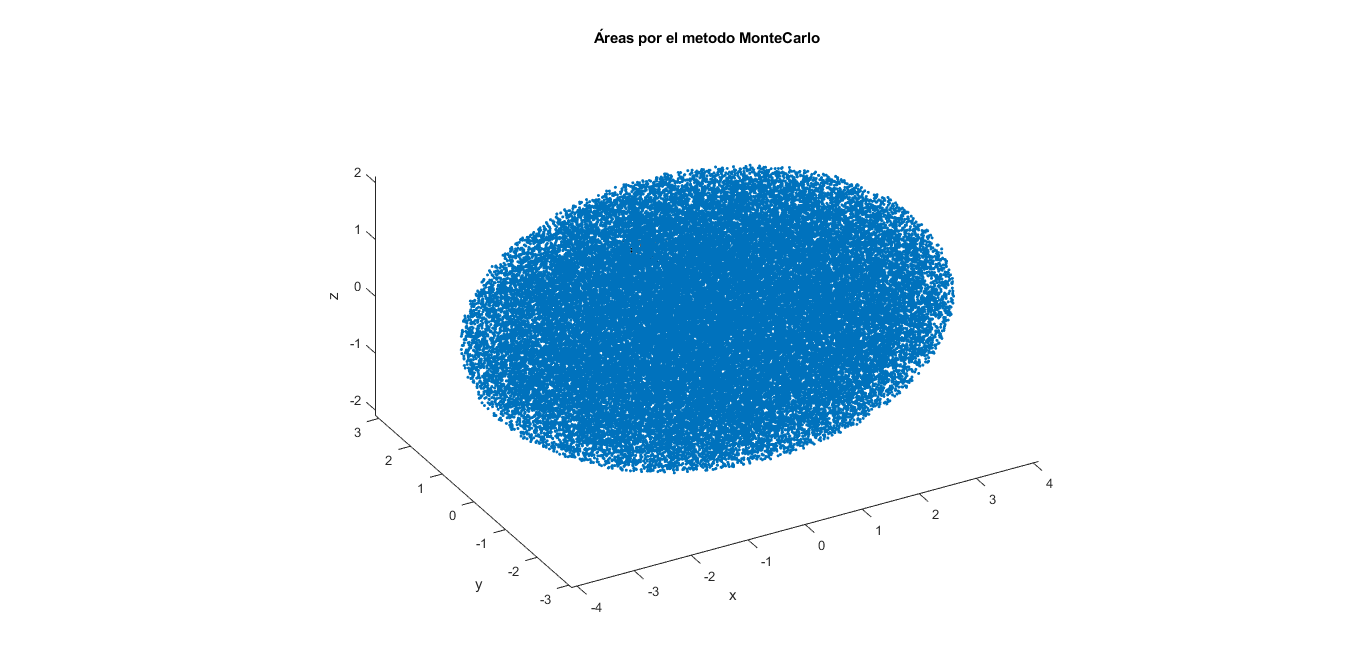
\includegraphics[width=1\textwidth]{images/FIG05A.png}
    \caption{Área de la sección - Vista general}
\end{figure}

\begin{figure}[H]
\centering
    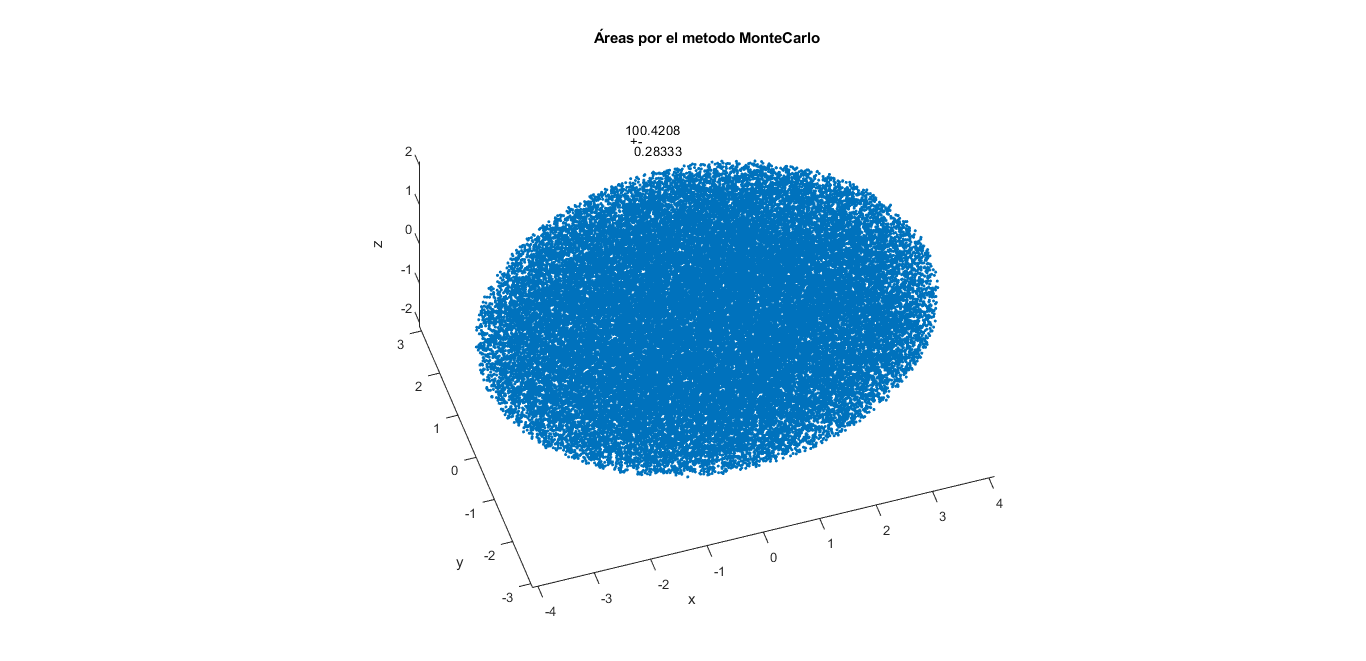
\includegraphics[width=1\textwidth]{images/FIG05B.png}
    \caption{Área de la sección - Vista general 2}
\end{figure}

\clearpage
\newpage

\begin{figure}[H]
\centering
    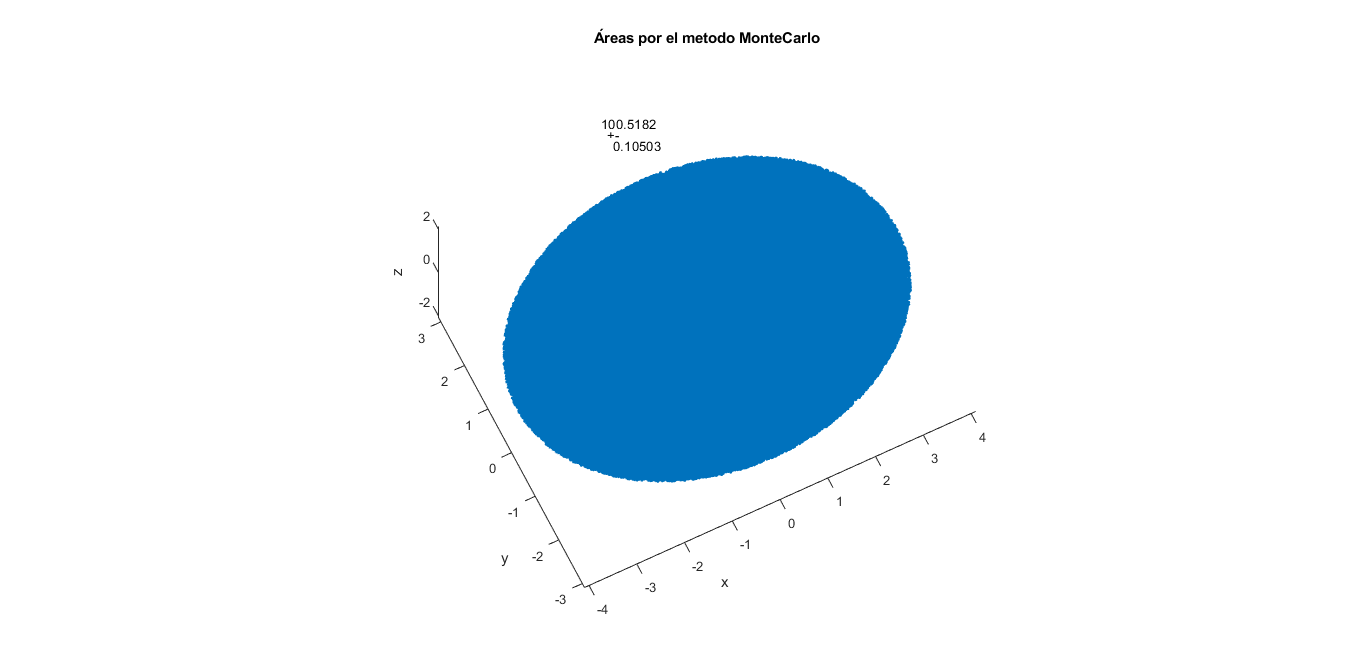
\includegraphics[width=1\textwidth]{images/FIG05C.png}
    \caption{Área de la sección - Vista general 3}
\end{figure}

El área de la sección es = $100.5182~+/-~0.10503$

\section{Encuentre el volumen del elipsoide en el primer cuadrante del problema 5}

\begin{lstlisting} [frame=single]
clear, clf, hold off
m = 100000; veces = 50;
ax = -4; bx  = 4;
ay = -3; by  = 3;
az = -2; bz  = 2; 
sa = 0; saa = 0;
for k=1:veces
    n=0;
    for i=1:m
        r = rand; x = ax + (bx-ax)*r;
        r = rand; y = ay + (by-ay)*r;
        r = rand; z = az + (bz-az)*r;
        if (x^2/16+y^2/9+z^2/4) < 1 && (x >=0) && (y >=0) && (z >=0) 
            n     = n+1;
            px(n) = x; 
            py(n) = y;
            pz(n) = z;
        end
    end
    volumen = n*(by-ay)*(bx-ax)*(bz-az)/m;
    sa   = sa + volumen;
    saa  = saa + volumen^2;
end
prom = sa/veces;
desv = sqrt(veces*saa-sa^2)/veces;
promedio = num2str(prom);
desviacion = num2str(desv);
plot3(px,py,pz,'.'),
title('Áreas por el metodo MonteCarlo') 
xlabel('x');
ylabel('y');
zlabel('z');
axis equal;
axis ([ax-0.1,bx+0.1,ay-0.1,by+0.1,az-0.1,bz+0.1]);
text(ax/2+bx/2,by-0.25+bz-0.25,promedio);
text(ax/2+bx/2,by-0.50+bz-0.25,'+-');
text(ax/2+bx/2,by-0.75+bz-0.25,desviacion);
\end{lstlisting}

\begin{figure}[H]
\centering
    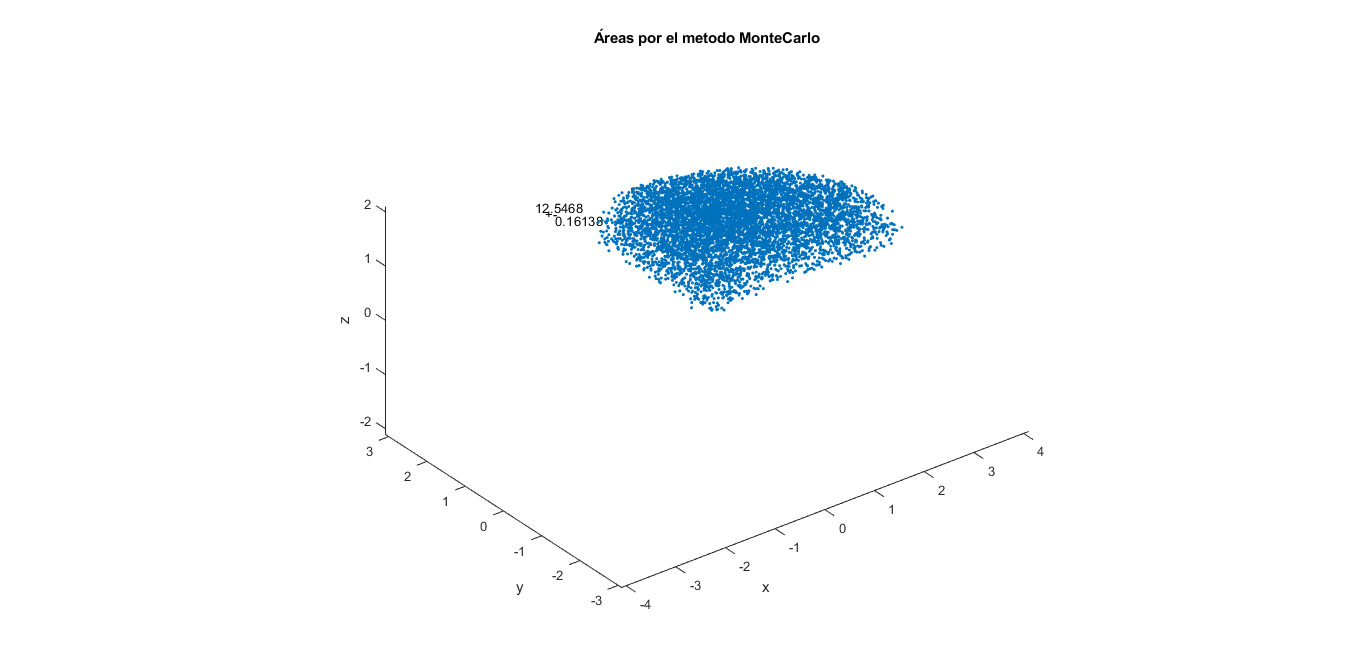
\includegraphics[width=0.9\textwidth]{images/FIG06A.png}
    \caption{Área de la sección - Vista general 1}
\end{figure}
\begin{figure}[H]
\centering
    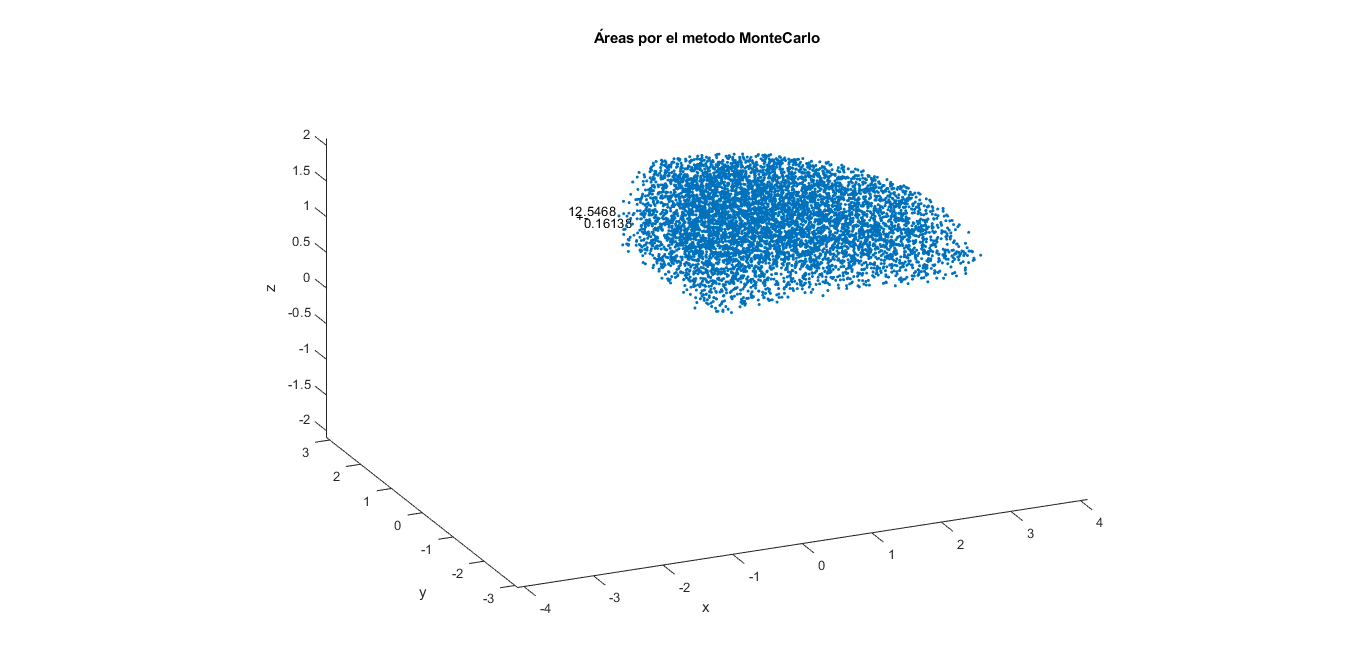
\includegraphics[width=0.9\textwidth]{images/FIG06B.png}
    \caption{Área de la sección - Vista general 2}
\end{figure}

El área de la sección es = $12.5468~+/-~0.16138$

\clearpage
\newpage

\section{Evalúe la integral}

\begin{equation}
\int_{0}^{\pi/2}\int_{0}^{\pi} sin(u)cos(v-\pi)~du~dv
\end{equation}

Primero realizaremos algunas gráficas para darnos una idea de lo que vamos a obtener en el código:

\begin{figure}[H]
\centering
    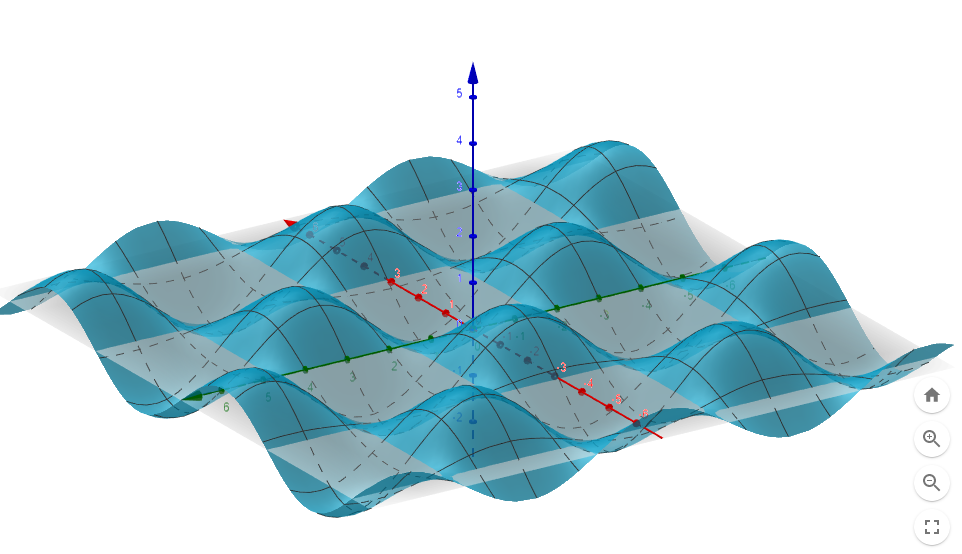
\includegraphics[width=0.5\textwidth]{images/Capture07.PNG}
    \caption{Gráfica de las líneas para delimitar el área del ejercicio 7}
\end{figure}

\begin{lstlisting} [frame=single]
clear, clf, hold off
m = 1000000; veces = 50;
ax = -3; bx  = 3;
ay = -3; by  = 3;
az = -3; bz  = 3; 
sa = 0; saa = 0;
for k=1:veces
    n=0;
    for i=1:m
        r = rand; x = ax + (bx-ax)*r;
        r = rand; y = ay + (by-ay)*r;
        r = rand; z = az + (bz-az)*r;
        if (sin(x)*(cos(y-pi)))<z && z <= 0&& (x>=0&&x<=pi) && (y>=0&&y<=(pi/2))
            n     = n+1;
            px(n) = x; 
            py(n) = y;
            pz(n) = z;
        end
    end
    volumen = n*(by-ay)*(bx-ax)*(bz-az)/m;
    sa   = sa + volumen;
    saa  = saa + volumen^2;
end
prom = sa/veces;
desv = sqrt(veces*saa-sa^2)/veces;
promedio = num2str(prom);
desviacion = num2str(desv);
plot3(px,py,pz,'.'),
title('Áreas por el metodo MonteCarlo') 
xlabel('x');
ylabel('y');
zlabel('z');
axis equal;
axis ([ax-0.1,bx+0.1,ay-0.1,by+0.1,az-0.1,bz+0.1]);
text(ax/2+bx/2,by-0.25+bz-0.25,promedio);
text(ax/2+bx/2,by-0.50+bz-0.25,'+-');
text(ax/2+bx/2,by-0.75+bz-0.25,desviacion);
\end{lstlisting}

\begin{figure}[H]
\centering
    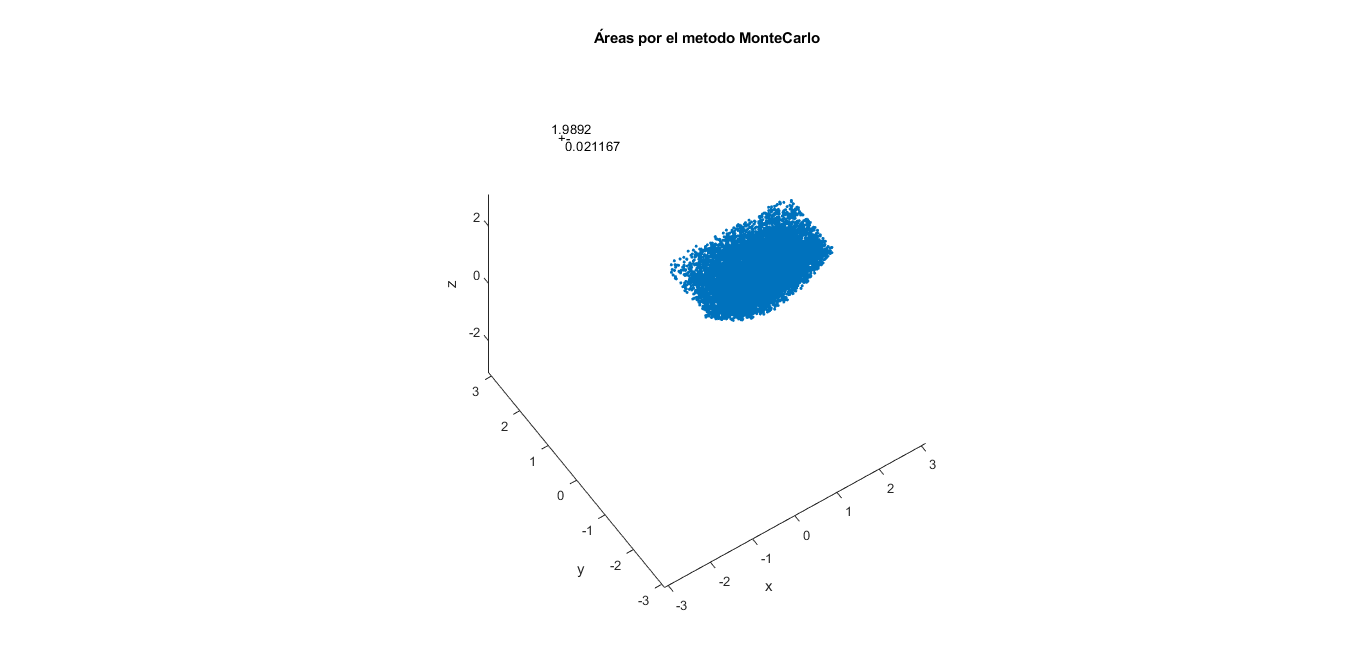
\includegraphics[width=1\textwidth]{images/FIG07A.png}
    \caption{Área de la sección - Vista general}
\end{figure}

\begin{figure}[H]
\centering
    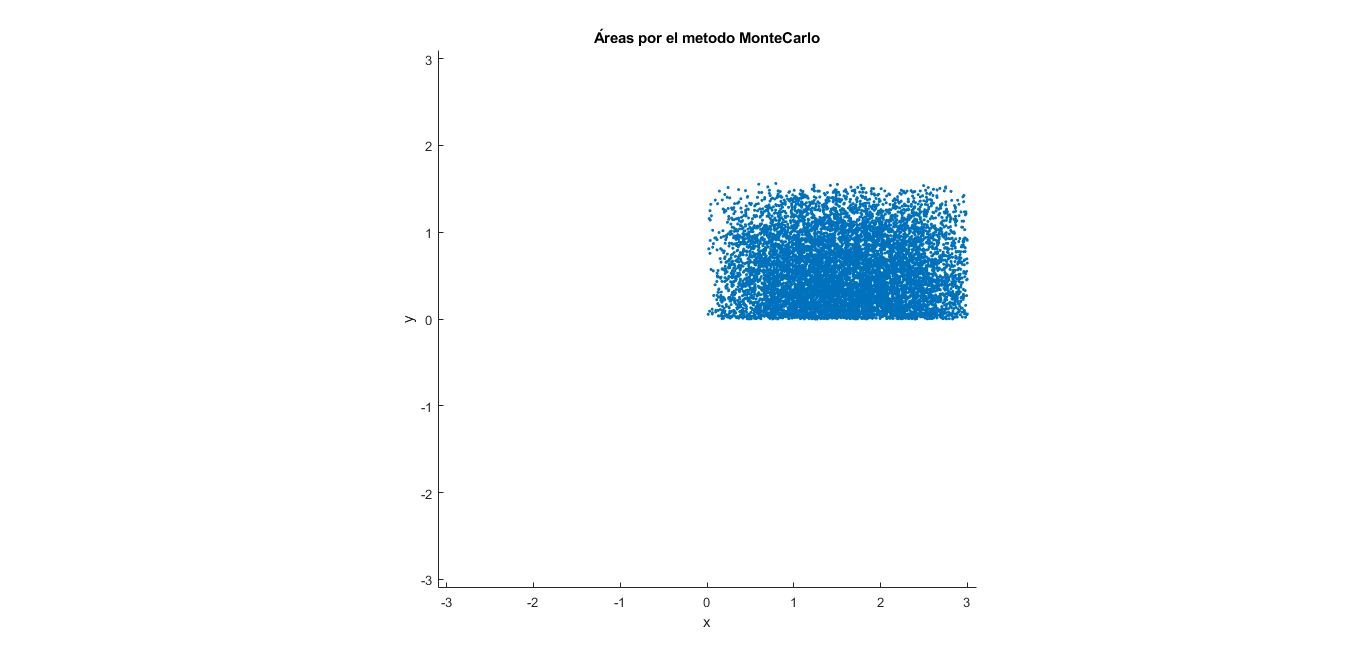
\includegraphics[width=1\textwidth]{images/FIG07B.png}
    \caption{Área de la sección - Vista general de los planos x e y}
\end{figure}

\clearpage
\newpage

\begin{figure}[H]
\centering
    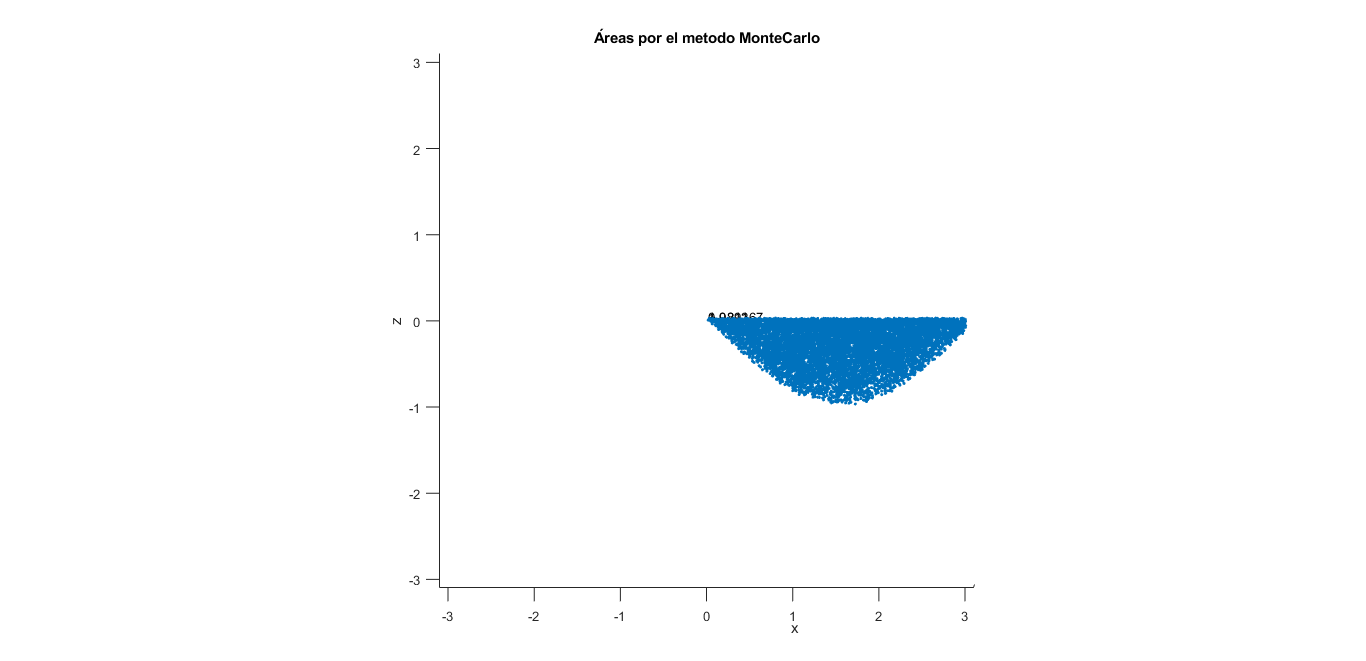
\includegraphics[width=1\textwidth]{images/FIG07C.png}
    \caption{Área de la sección - Vista general de los planos x e z}
\end{figure}

\begin{figure}[H]
\centering
    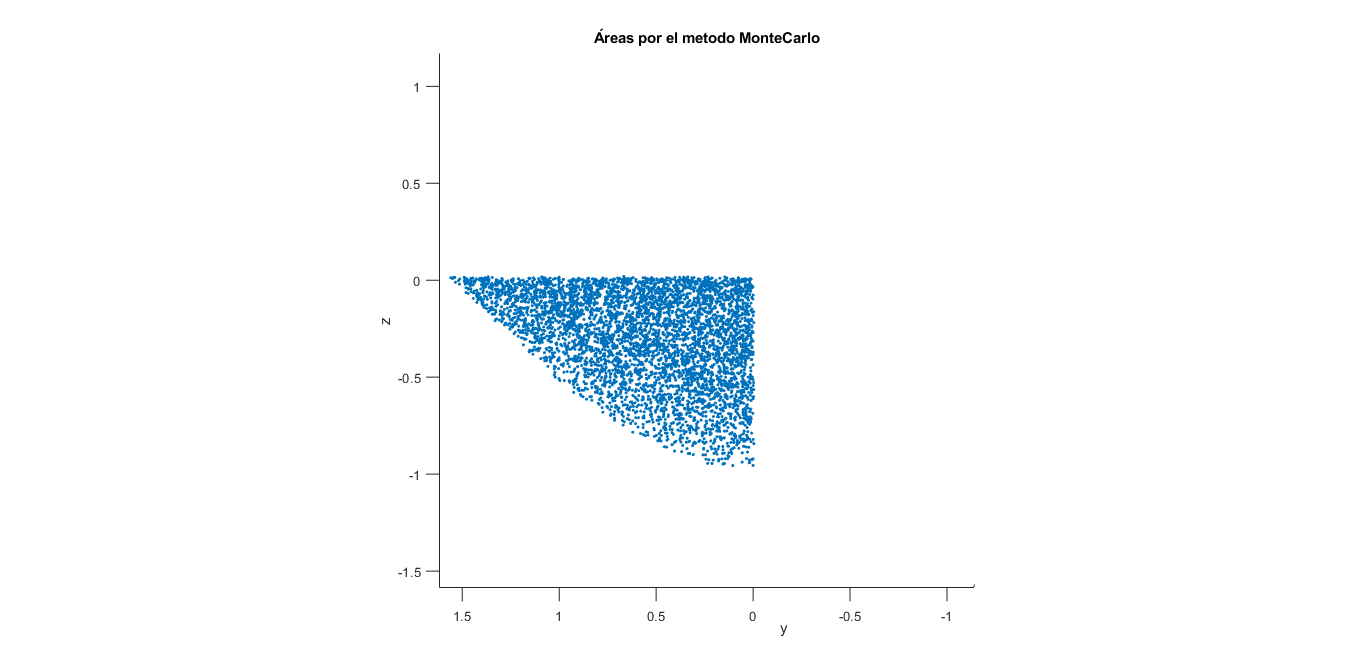
\includegraphics[width=1\textwidth]{images/FIG07D.png}
    \caption{Área de la sección - Vista general de los planos y e z}
\end{figure}

El área de la sección es = $1.9892~+/-~0.021167$

\section{Evalúe la integral}

\begin{equation}
\iint \limits_{D}^{~}\frac{2y-1}{2x+1}~dx~dy
\end{equation}

En el dominio:

\begin{equation}
x=0
\end{equation}
\begin{equation}
y=0
\end{equation}
\begin{equation}
2x-y=4
\end{equation}

\begin{lstlisting} [frame=single]
clear, clf, hold off
m = 100000; veces = 50;
ax = -3; bx  = 5;
ay = -3; by  = 5;
az = -3; bz  = 10; 
sa = 0; saa = 0;
for k=1:veces
    n=0;
    for i=1:m
        r = rand; x = ax + (bx-ax)*r;
        r = rand; y = ay + (by-ay)*r;
        r = rand; z = az + (bz-az)*r;
        if ((2*y-1)/(2*x+1)>=z&&(2*x-y)<=4) && (x>=0) && (y>=0)
            n     = n+1;
            px(n) = x; 
            py(n) = y;
            pz(n) = z;
        end
    end
    volumen = n*(by-ay)*(bx-ax)*(bz-az)/m;
    sa   = sa + volumen;
    saa  = saa + volumen^2;
end
prom = sa/veces;
desv = sqrt(veces*saa-sa^2)/veces;
promedio = num2str(prom);
desviacion = num2str(desv);
plot3(px,py,pz,'.'),
title('Áreas por el metodo MonteCarlo') 
xlabel('x');
ylabel('y');
zlabel('z');
axis equal;
axis ([ax-0.1,bx+0.1,ay-0.1,by+0.1,az-0.1,bz+0.1]);
text(ax/2+bx/2,by-0.25+bz-0.25,promedio);
text(ax/2+bx/2,by-0.50+bz-0.5,'+-');
text(ax/2+bx/2,by-0.75+bz-0.75,desviacion);
\end{lstlisting}



\begin{figure}[H]
\centering
    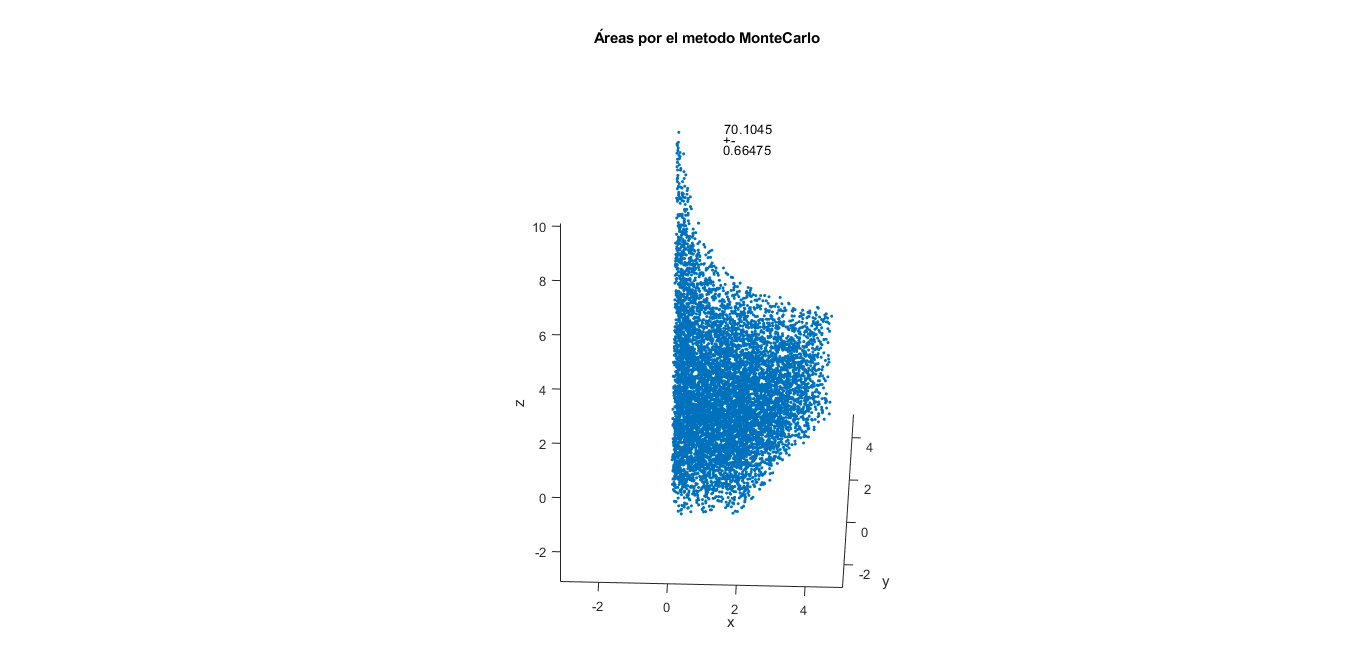
\includegraphics[width=1\textwidth]{images/FIG08A.png}
    \caption{Área de la sección - Vista general}
\end{figure}

\begin{figure}[H]
\centering
    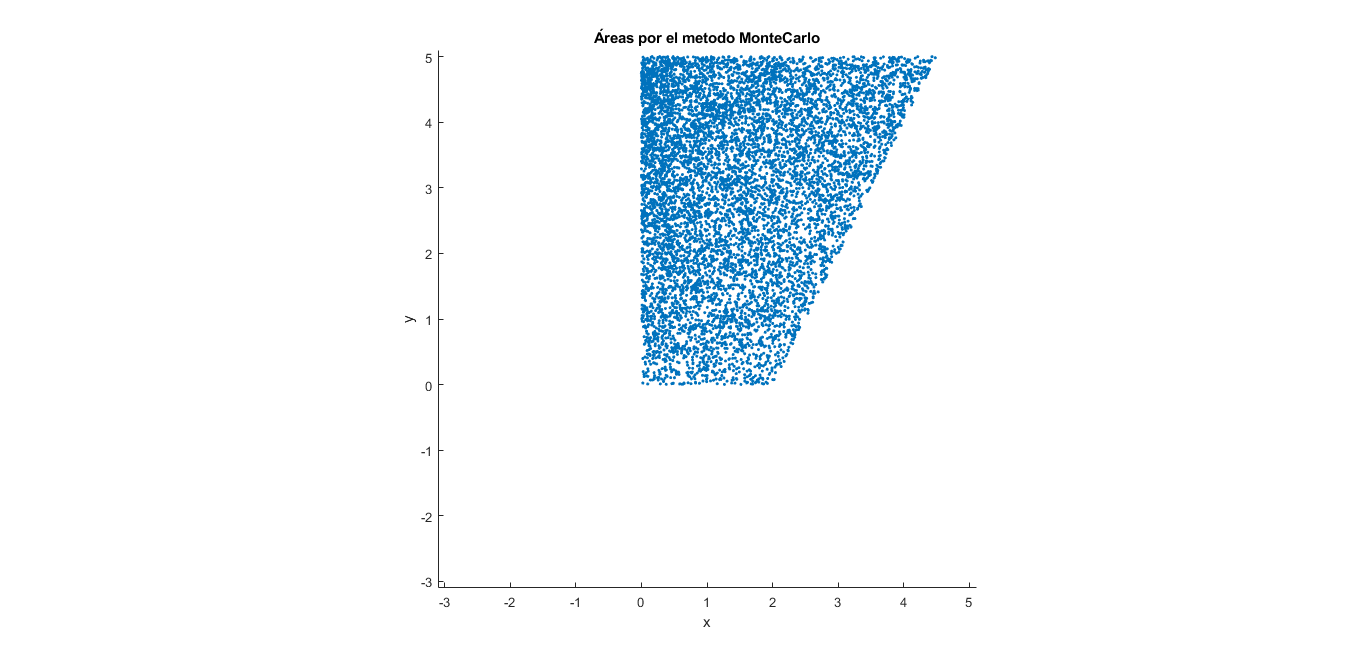
\includegraphics[width=1\textwidth]{images/FIG08B.png}
    \caption{Área de la sección - Vista general de los planos x e y}
\end{figure}

\clearpage
\newpage

\begin{figure}[H]
\centering
    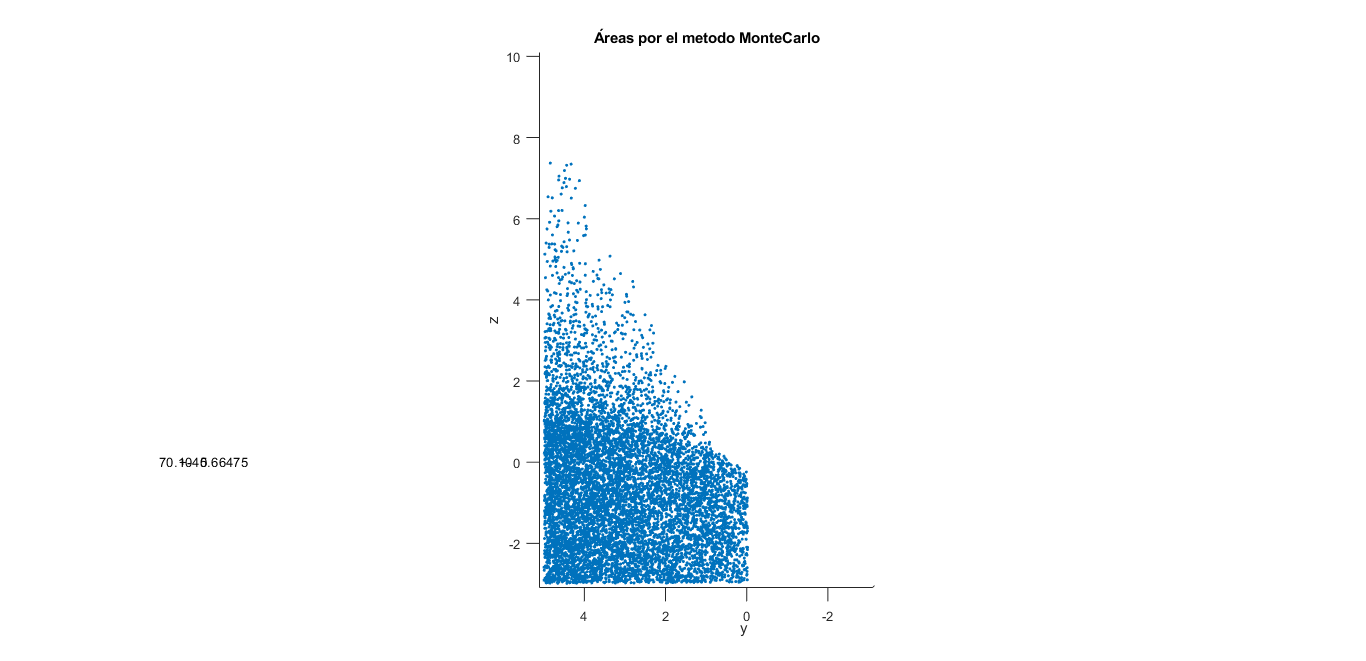
\includegraphics[width=1\textwidth]{images/FIG08C.png}
    \caption{Área de la sección - Vista general de los planos x e z}
\end{figure}

\begin{figure}[H]
\centering
    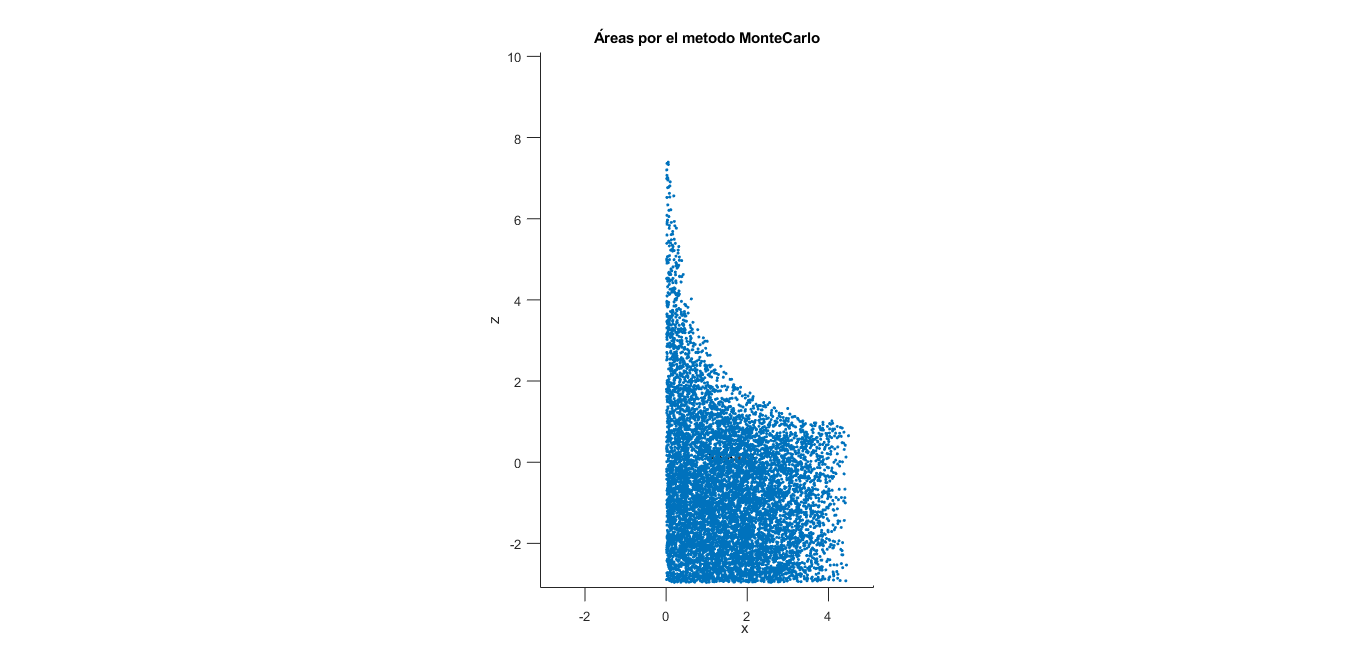
\includegraphics[width=1\textwidth]{images/FIG08D.png}
    \caption{Área de la sección - Vista general de los planos y e z}
\end{figure}

El área de la sección es = $70.1045~+/-~0.66475$

%%%%%%%%%%%%%%%%%%%%%%%%%%%%%%%%%5

\section{Evalúe la integral}
Para $n=3$.
\begin{equation}
\iint \limits_{D}^{~}x^ny^n~dx~dy
\end{equation}

En el dominio:

\begin{equation}
y=x^2
\end{equation}
\begin{equation}
x=y^2
\end{equation}

\begin{lstlisting} [frame=single]
clear, clf, hold off
m = 100000; veces = 50;
ax = -3; bx  = 5;
ay = -3; by  = 5;
az = -3; bz  = 10; 
sa = 0; saa = 0;
for k=1:veces
    n=0;
    for i=1:m
        r = rand; x = ax + (bx-ax)*r;
        r = rand; y = ay + (by-ay)*r;
        r = rand; z = az + (bz-az)*r;
        if (( x^3*y^3)>=z && (x^2)<=y && (y^2)<=x )
            n     = n+1;
            px(n) = x; 
            py(n) = y;
            pz(n) = z;
        end
    end
    volumen = n*(by-ay)*(bx-ax)*(bz-az)/m;
    sa   = sa + volumen;
    saa  = saa + volumen^2;
end
prom = sa/veces;
desv = sqrt(veces*saa-sa^2)/veces;
promedio = num2str(prom);
desviacion = num2str(desv);
plot3(px,py,pz,'.'),
title('Áreas por el metodo MonteCarlo') 
xlabel('x');
ylabel('y');
zlabel('z');
axis equal;
axis ([ax-0.1,bx+0.1,ay-0.1,by+0.1,az-0.1,bz+0.1]);
text(ax/2+bx/2,by-0.25+bz-0.25,promedio);
text(ax/2+bx/2,by-0.50+bz-0.5,'+-');
text(ax/2+bx/2,by-0.75+bz-0.75,desviacion);
\end{lstlisting}



\begin{figure}[H]
\centering
    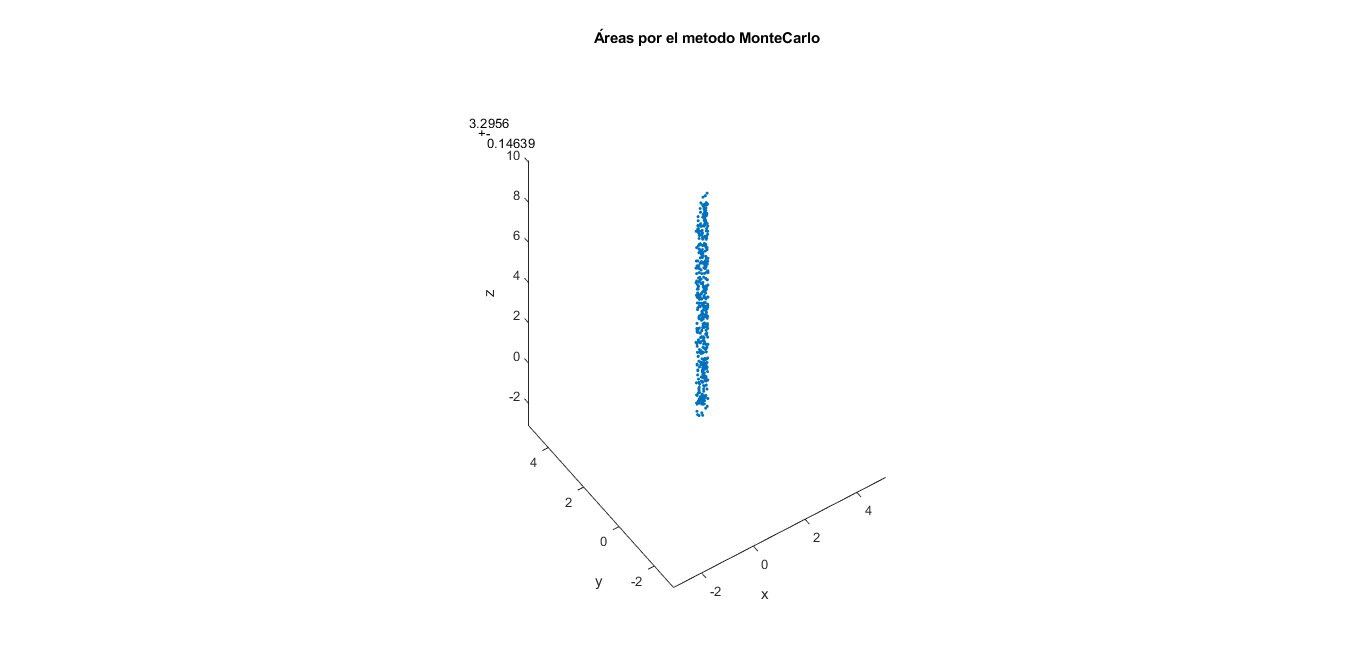
\includegraphics[width=1\textwidth]{images/FIG09A.png}
    \caption{Área de la sección - Vista general}
\end{figure}

\begin{figure}[H]
\centering
    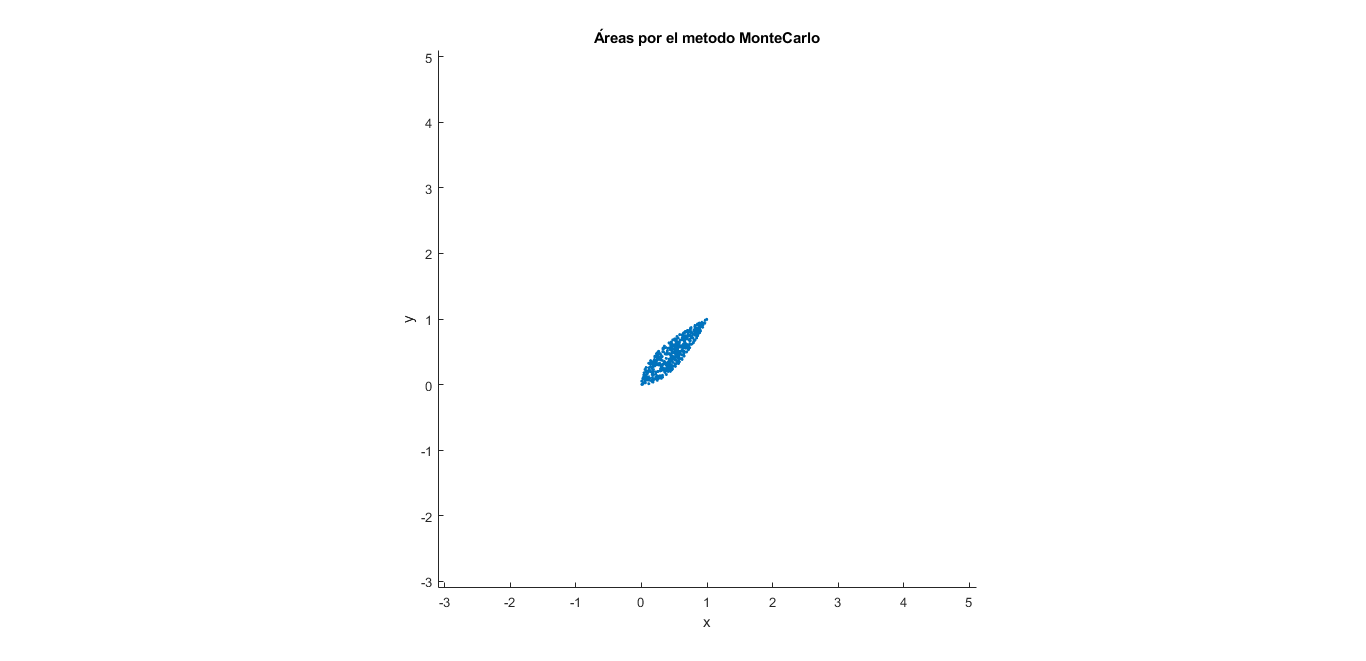
\includegraphics[width=1\textwidth]{images/FIG09B.png}
    \caption{Área de la sección - Vista general de los planos x e y}
\end{figure}

\clearpage
\newpage

\begin{figure}[H]
\centering
    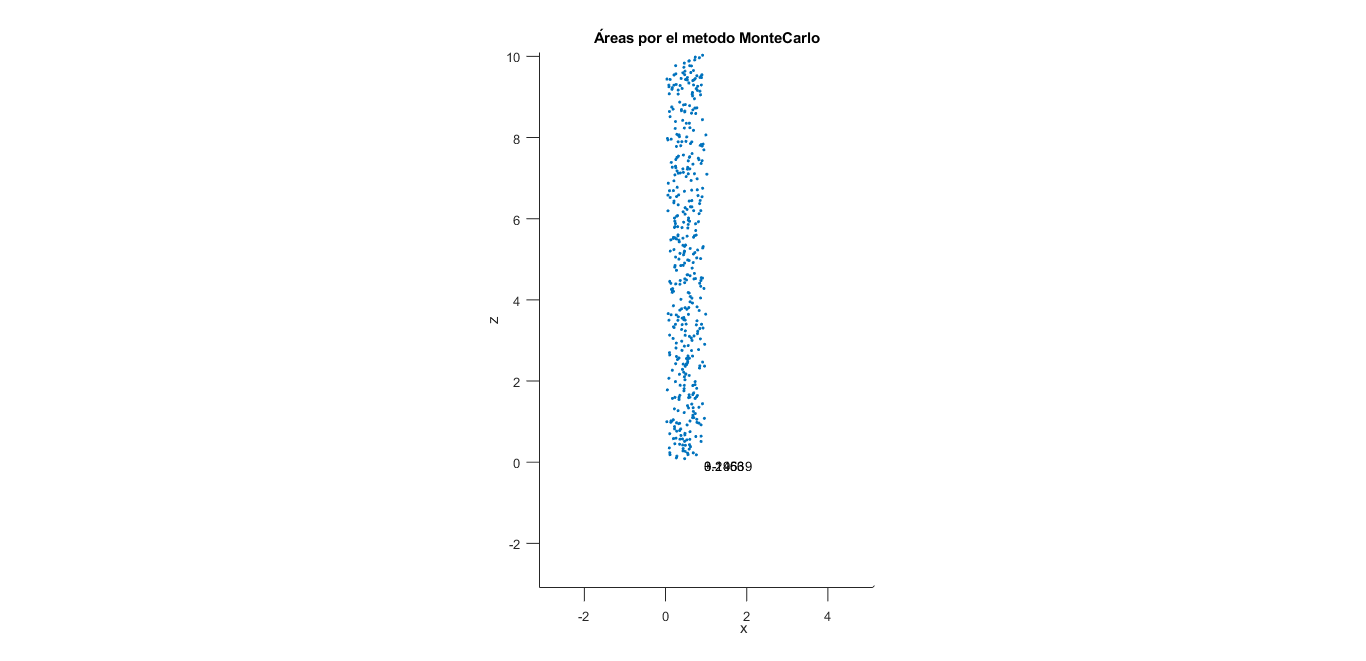
\includegraphics[width=1\textwidth]{images/FIG09C.png}
    \caption{Área de la sección - Vista general de los planos x e z}
\end{figure}

\begin{figure}[H]
\centering
    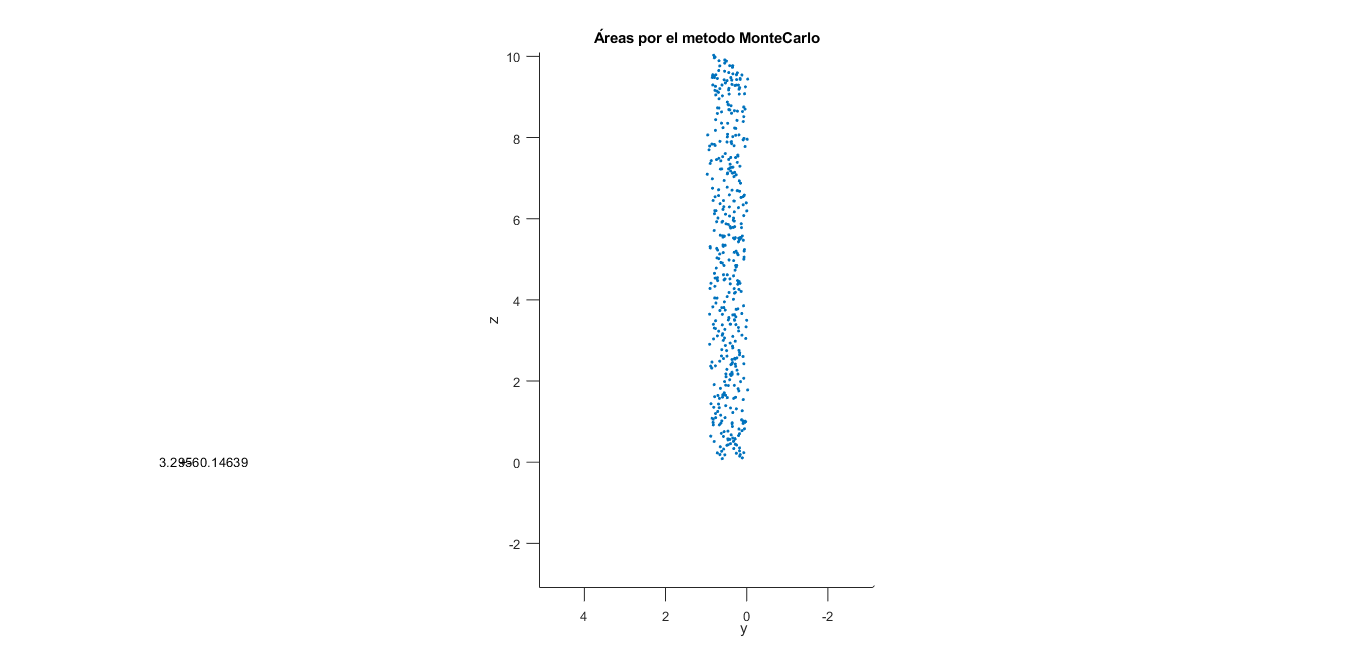
\includegraphics[width=1\textwidth]{images/FIG09D.png}
    \caption{Área de la sección - Vista general de los planos y e z}
\end{figure}

El área de la sección es = $3.2956~+/-~0.14639$



\end{document}